\begin{figure}[H]
    \centering
    \includegraphics[width=\textwidth]{img/Analisis/DiagramaProcesos/DiagramaProceso01_Captura Parámetros.png}
    \caption{Diagrama de Proceso Interno 01: Captura de Paráametros}%
    \label{fig:process_diagram01}
\end{figure}

\begin{figure}[H]
    \centering
    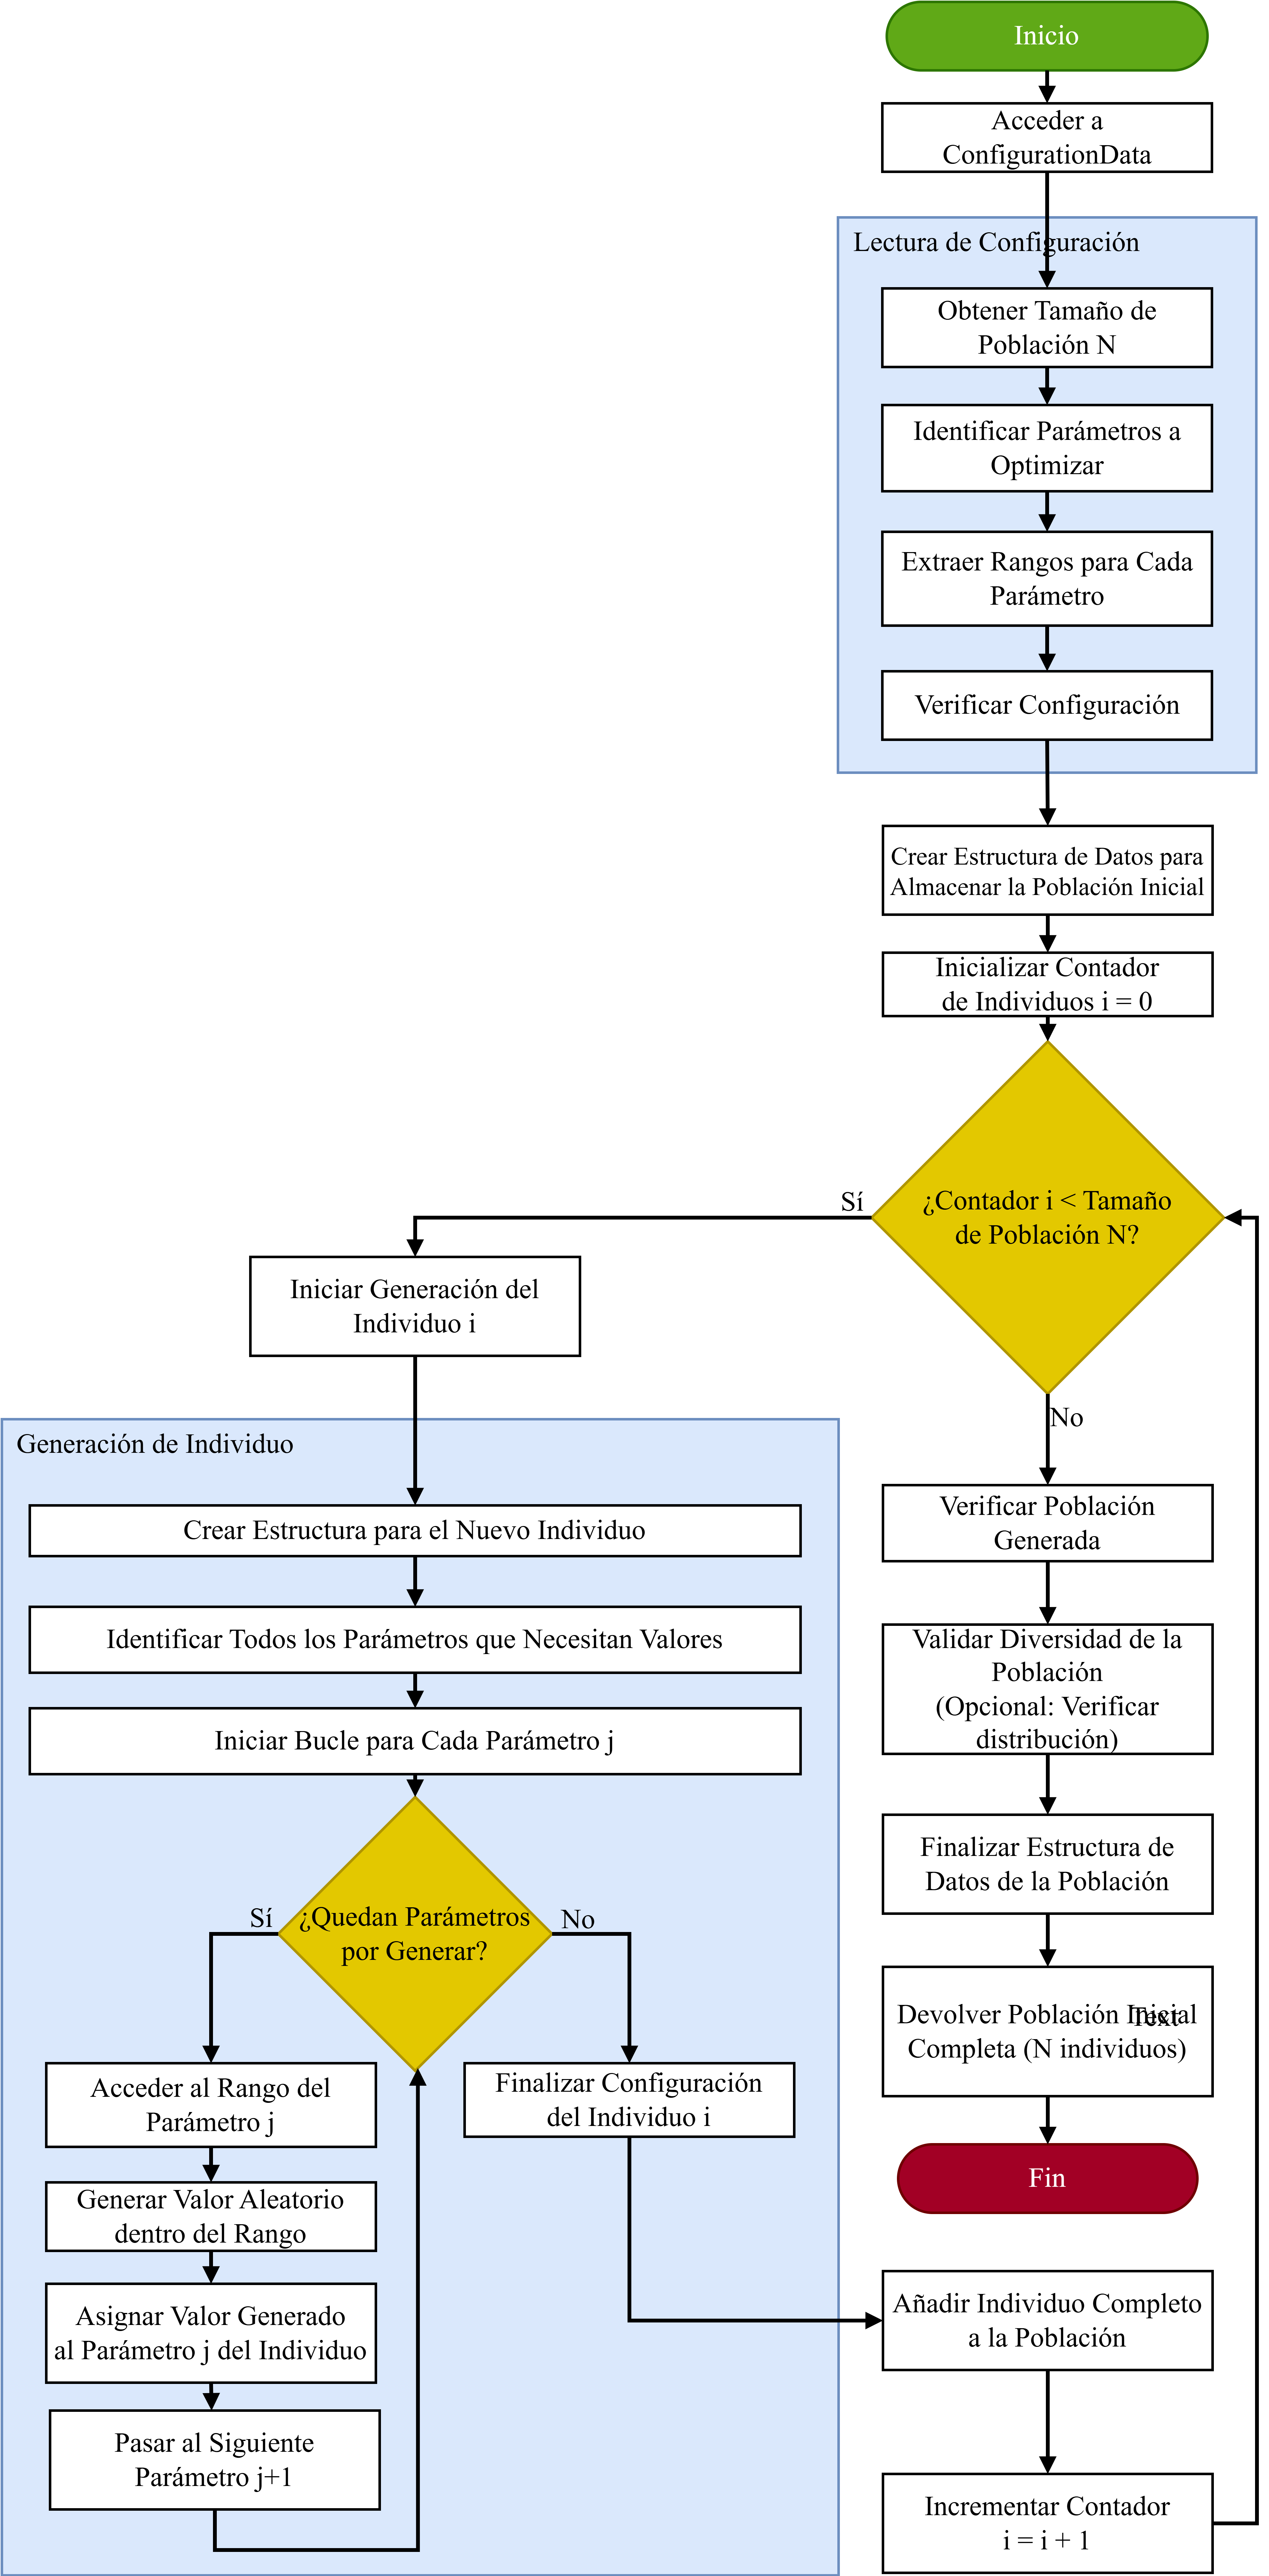
\includegraphics[width=\textwidth]{img/Analisis/DiagramaProcesos/DiagramaProceso02_InicializarPoblacion.png}
    \caption{Diagrama de Proceso Interno 02: Inicializar Población}%
    \label{fig:process_diagram02}
\end{figure}

\begin{figure}[H]
    \centering
    \includegraphics[width=\textwidth]{img/Analisis/DiagramaProcesos/DiagramaProceso03_GenerarNuevaGeneración.png}
    \caption{Diagrama de Proceso Interno 03: Generar Nueva Generación}%
    \label{fig:process_diagram03}
\end{figure}

\begin{figure}[H]
    \centering
    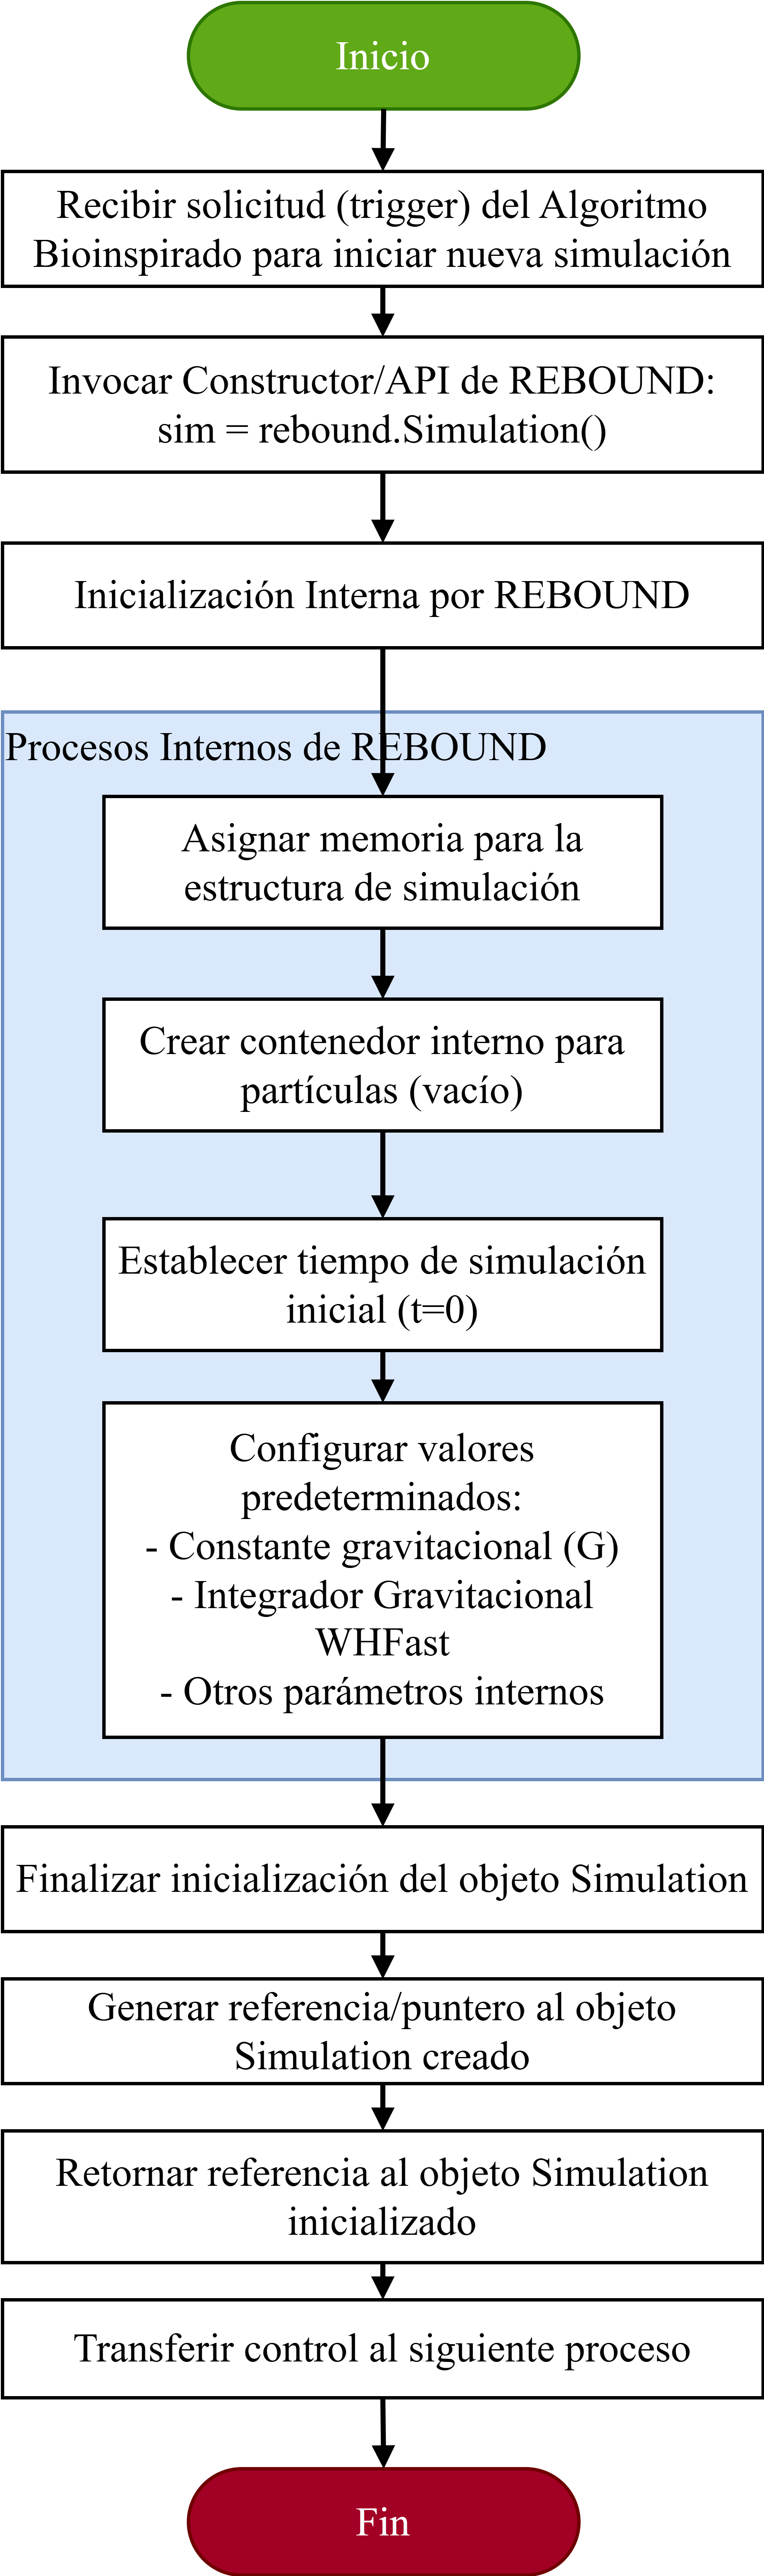
\includegraphics[width=\textwidth]{img/Analisis/DiagramaProcesos/DiagramaProceso04_CrearSimulacion.png}
    \caption{Diagrama de Proceso Interno 04: Crear Simulación}%
    \label{fig:process_diagram04}
\end{figure}

\begin{figure}[H]
    \centering
    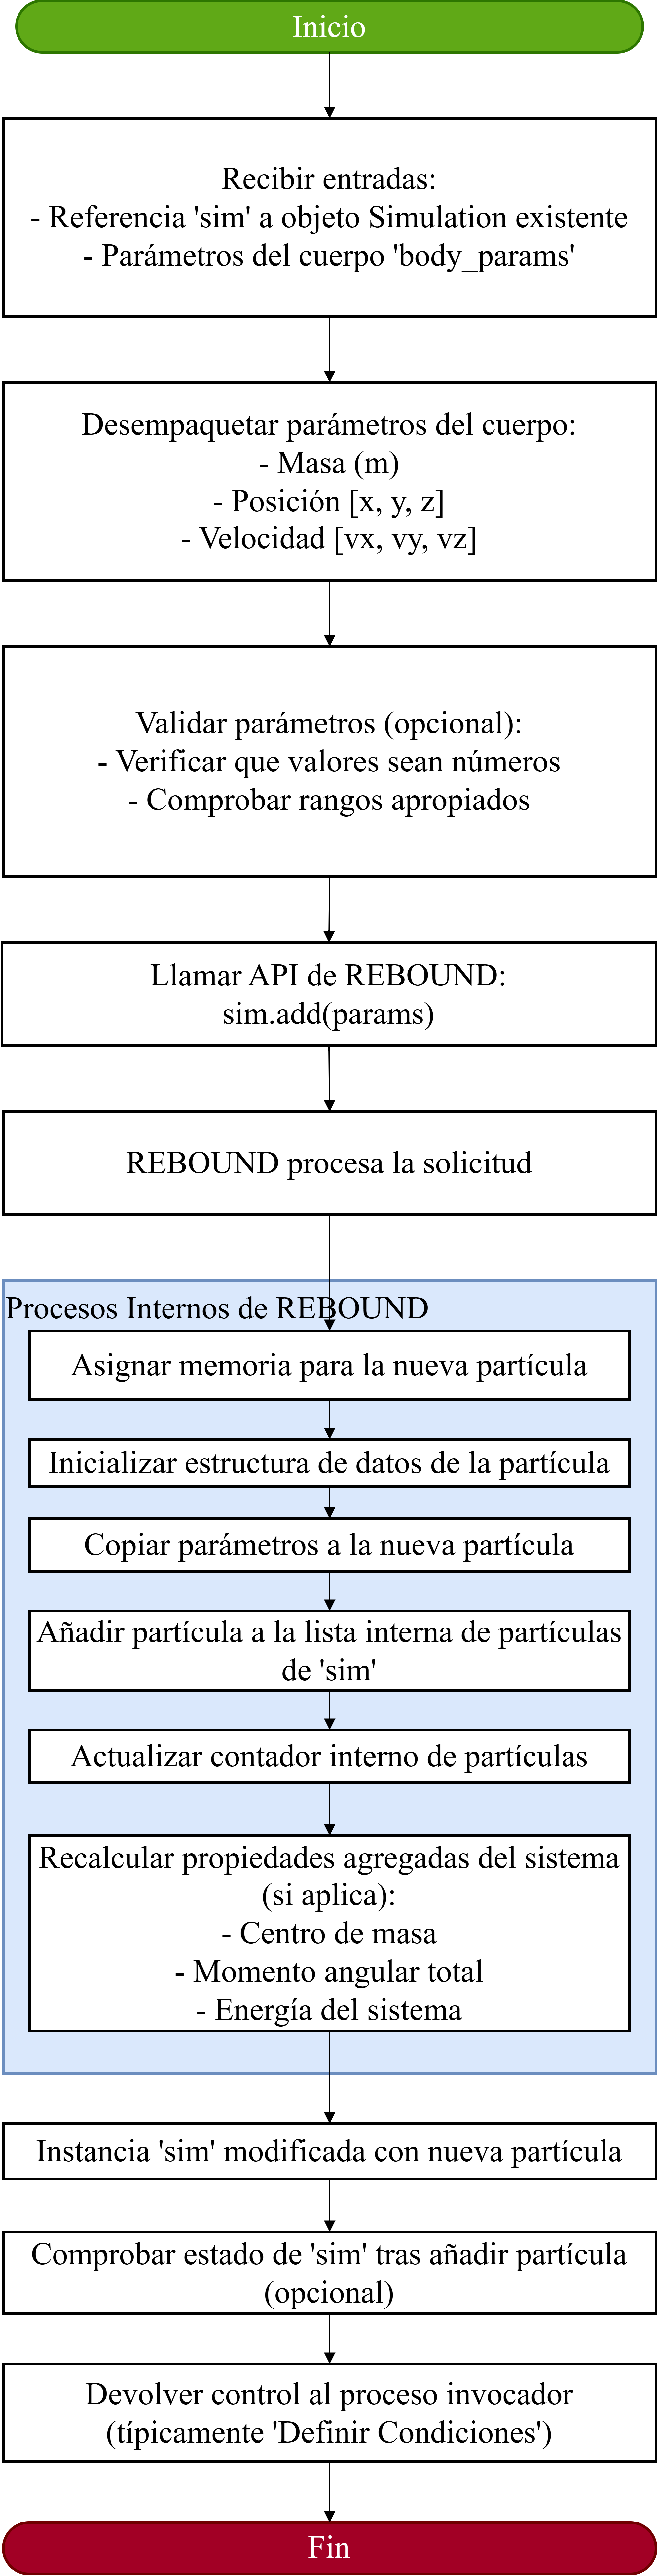
\includegraphics[width=\textwidth]{img/Analisis/DiagramaProcesos/DiagramaProceso05AgregarCuerpos.png}
    \caption{Diagrama de Proceso Interno 05: Agregar Cuerpos}%
    \label{fig:process_diagram05}
\end{figure}

\begin{figure}[H]
    \centering
    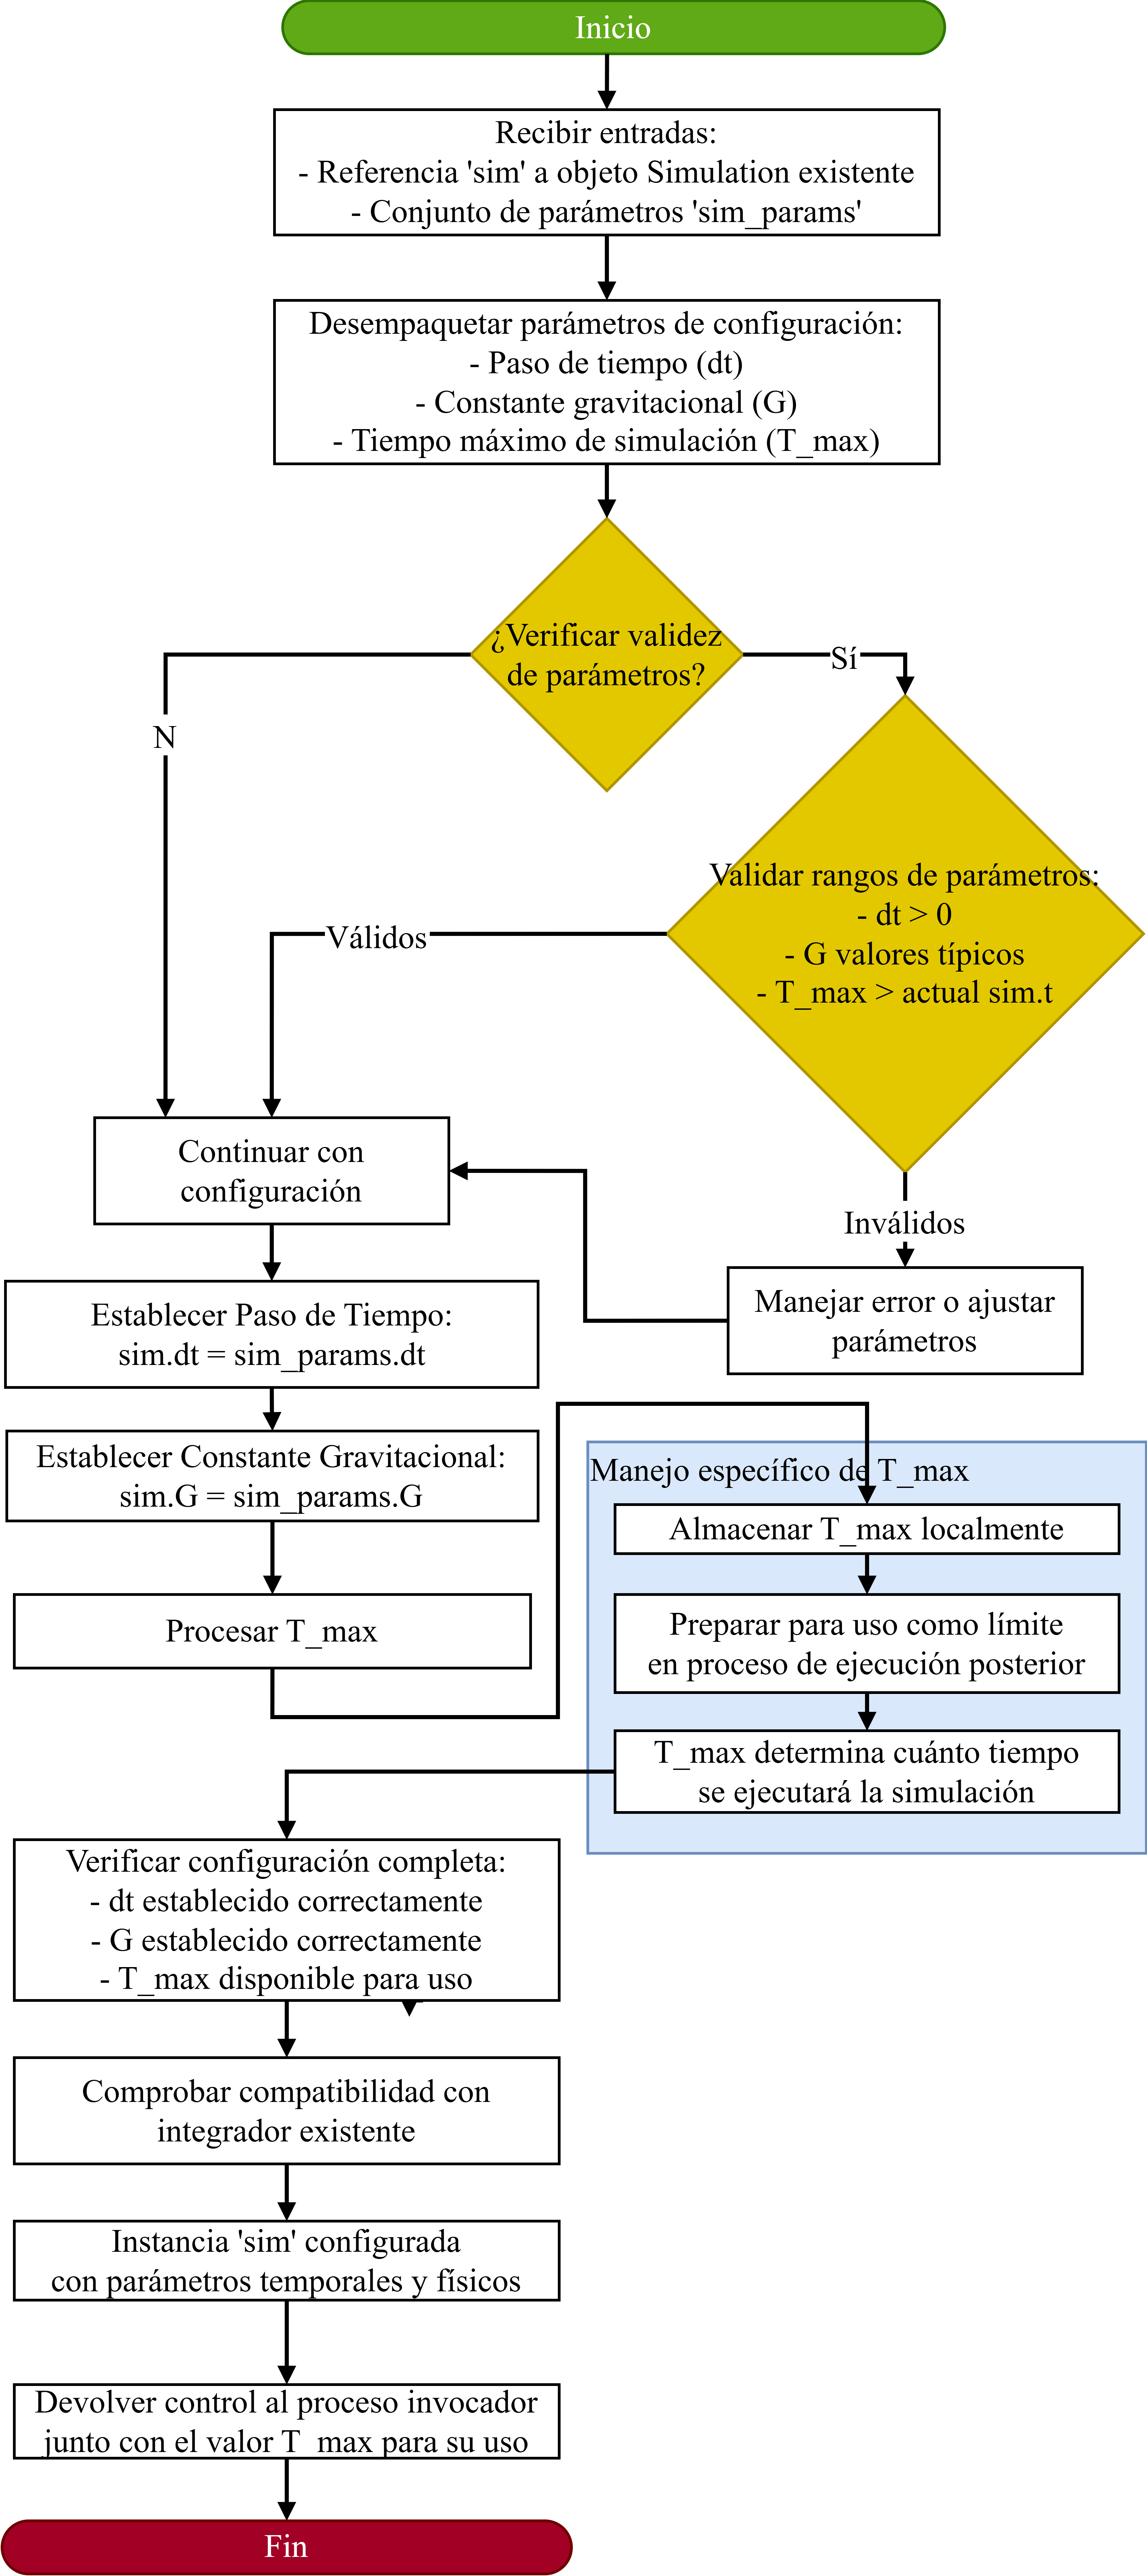
\includegraphics[width=\textwidth]{img/Analisis/DiagramaProcesos/DiagramaProceso06_DefinirCondiciones.png}
    \caption{Diagrama de Proceso Interno 06: Definir Condiciones}%
    \label{fig:process_diagram06}
\end{figure}

\begin{figure}[H]
    \centering
    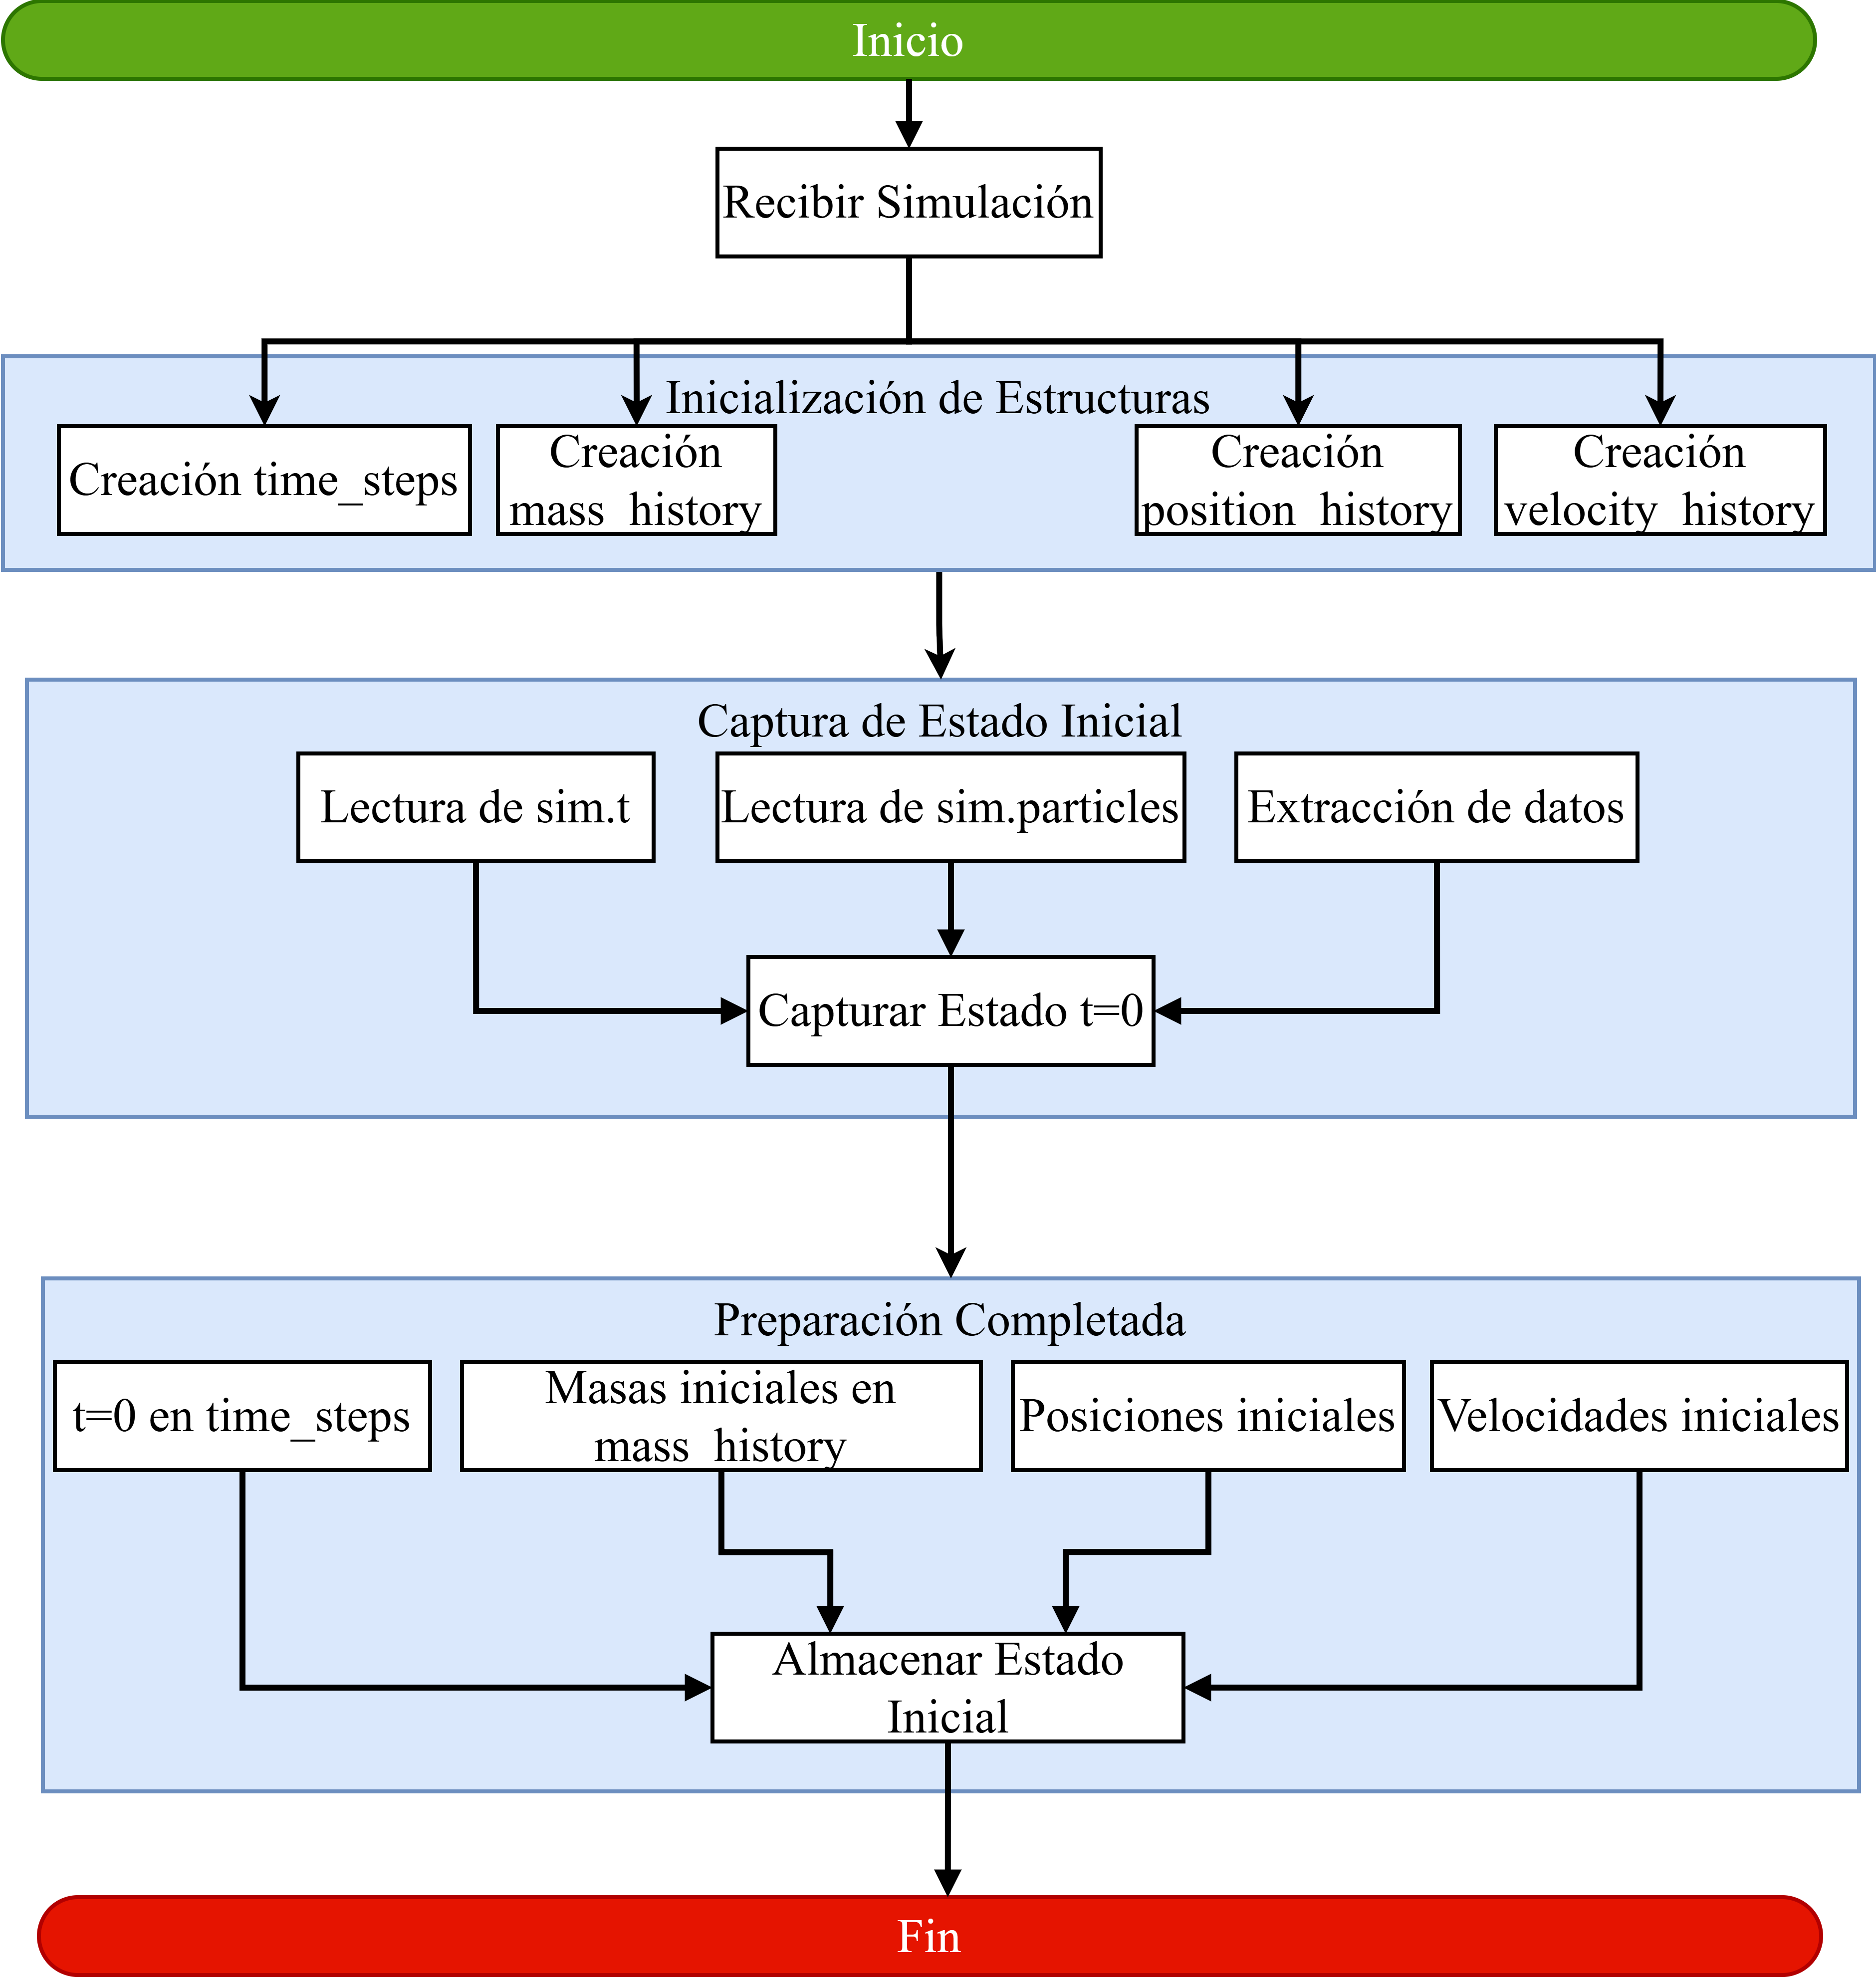
\includegraphics[width=\textwidth]{img/Analisis/DiagramaProcesos/DiagramaProceso07_IniciarSimulacion.png}
    \caption{Diagrama de Proceso Interno 07: Iniciar Simulación}%
    \label{fig:process_diagram07}
\end{figure}

\begin{figure}[H]
    \centering
    \includegraphics[width=\textwidth]{img/Analisis/DiagramaProcesos/DiagramaProceso08_ResolverEcuaciones.png}
    \caption{Diagrama de Proceso Interno 08: Resolver Ecuaciones}%
    \label{fig:process_diagram08}
\end{figure}

\begin{figure}[H]
    \centering
    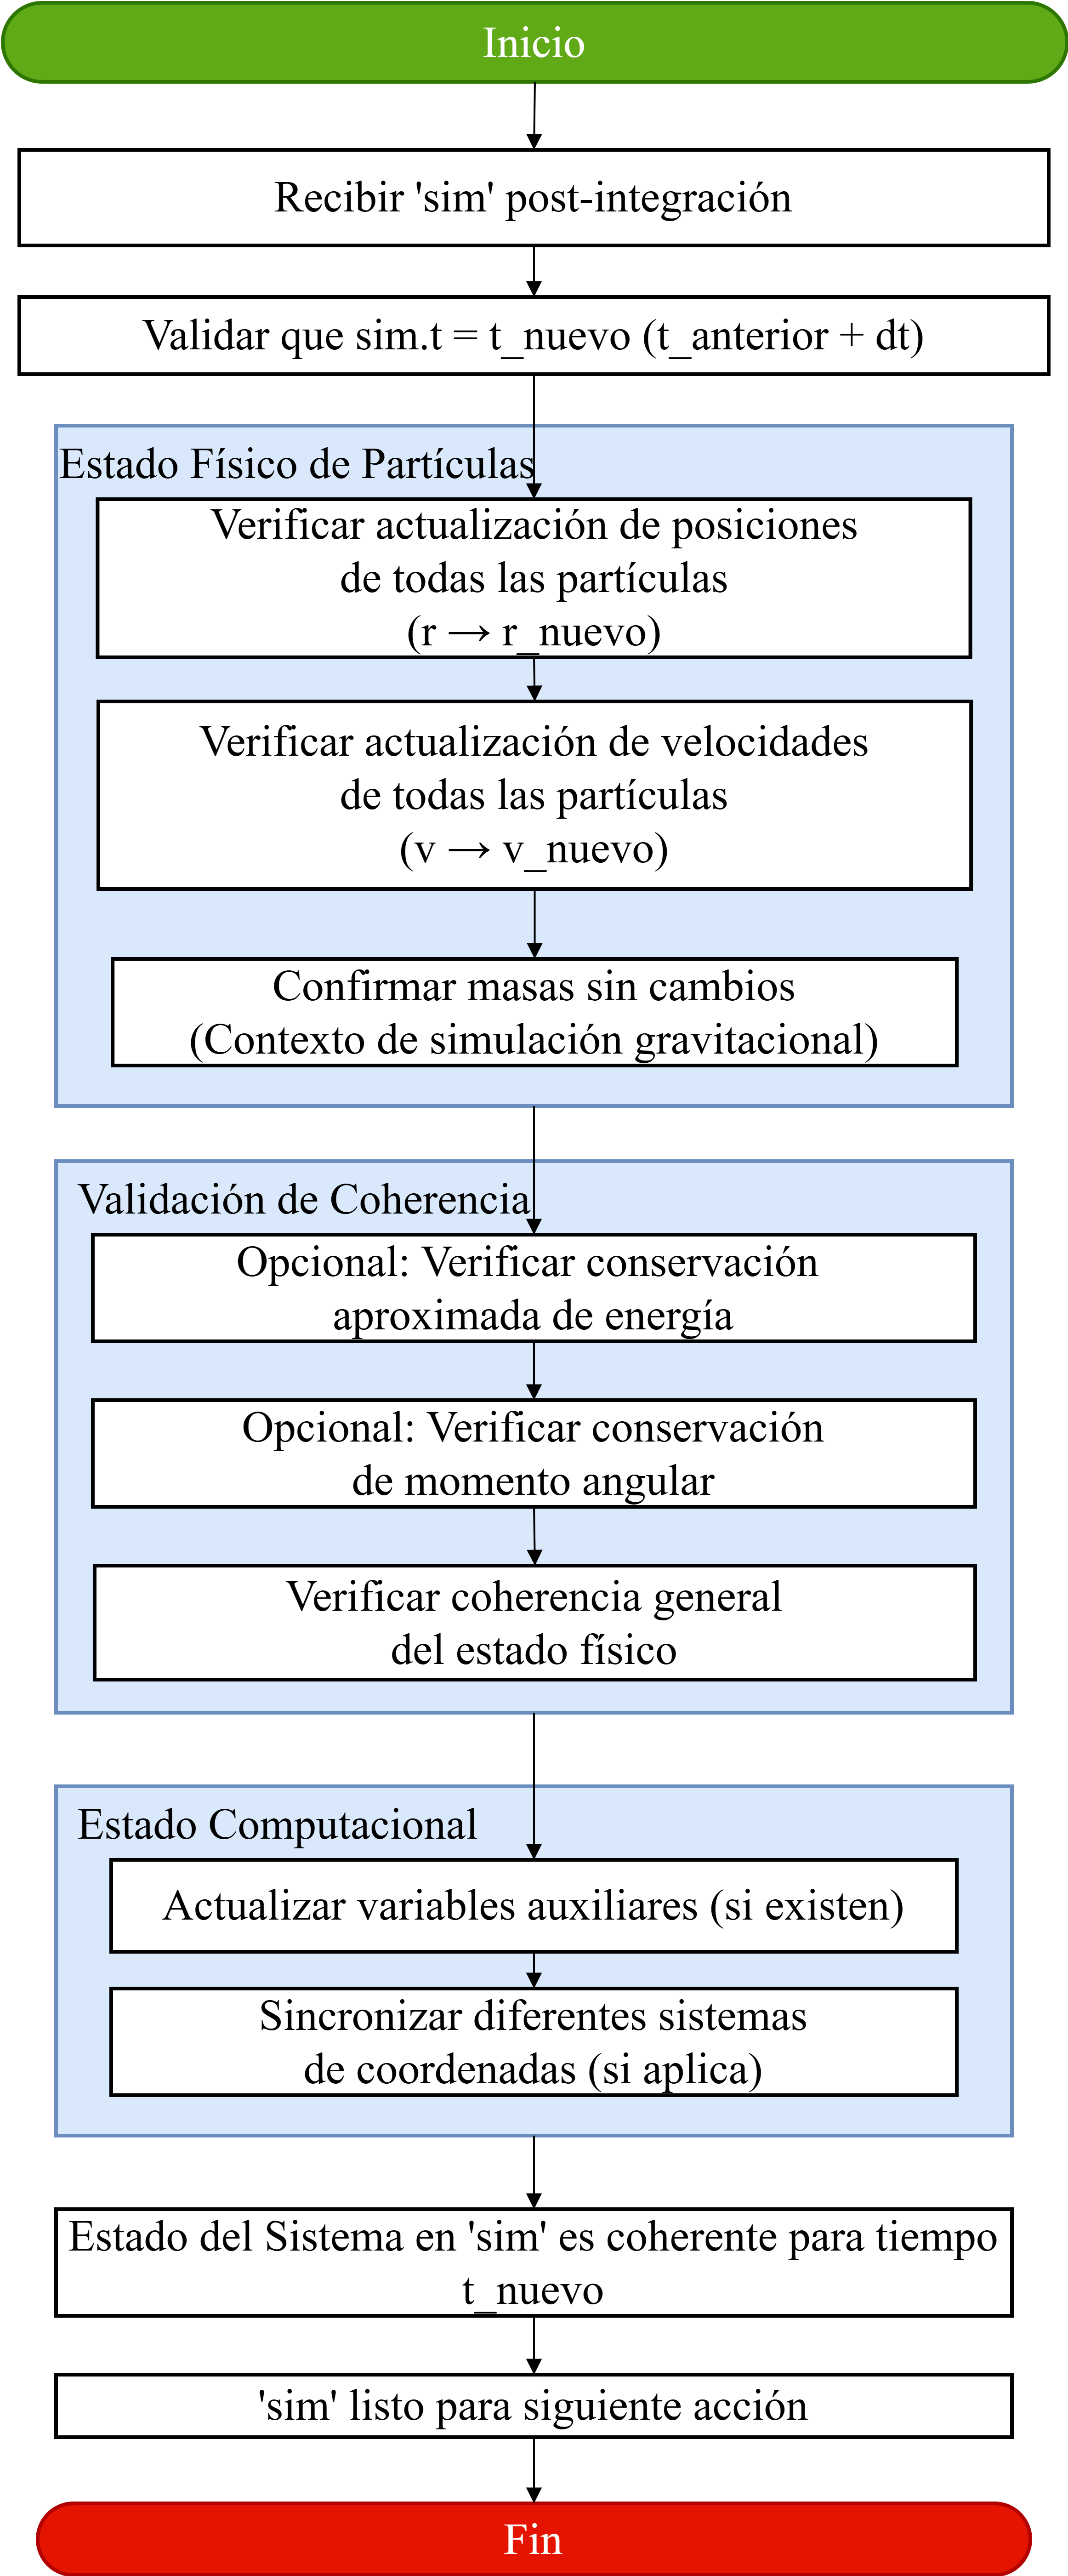
\includegraphics[width=\textwidth]{img/Analisis/DiagramaProcesos/DiagramaProceso09_ActualizarEstado.png}
    \caption{Diagrama de Proceso Interno 09: Actualizar Estado}%
    \label{fig:process_diagram09}
\end{figure}

\begin{figure}[H]
    \centering
    \includegraphics[width=\textwidth]{img/Analisis/DiagramaProcesos/DiagramaProceso10_RecolectarDatos.png}
    \caption{Diagrama de Proceso Interno 10: Recolectar Datos}%
    \label{fig:process_diagram10}
\end{figure}

\begin{figure}[H]
    \centering
    \includegraphics[width=\textwidth]{img/Analisis/DiagramaProcesos/DiagramaProceso011_ProcesarDatos.png}
    \caption{Diagrama de Proceso Interno 11: Procesa Datos}%
    \label{fig:process_diagram11}
\end{figure}

\begin{figure}[H]
    \centering
    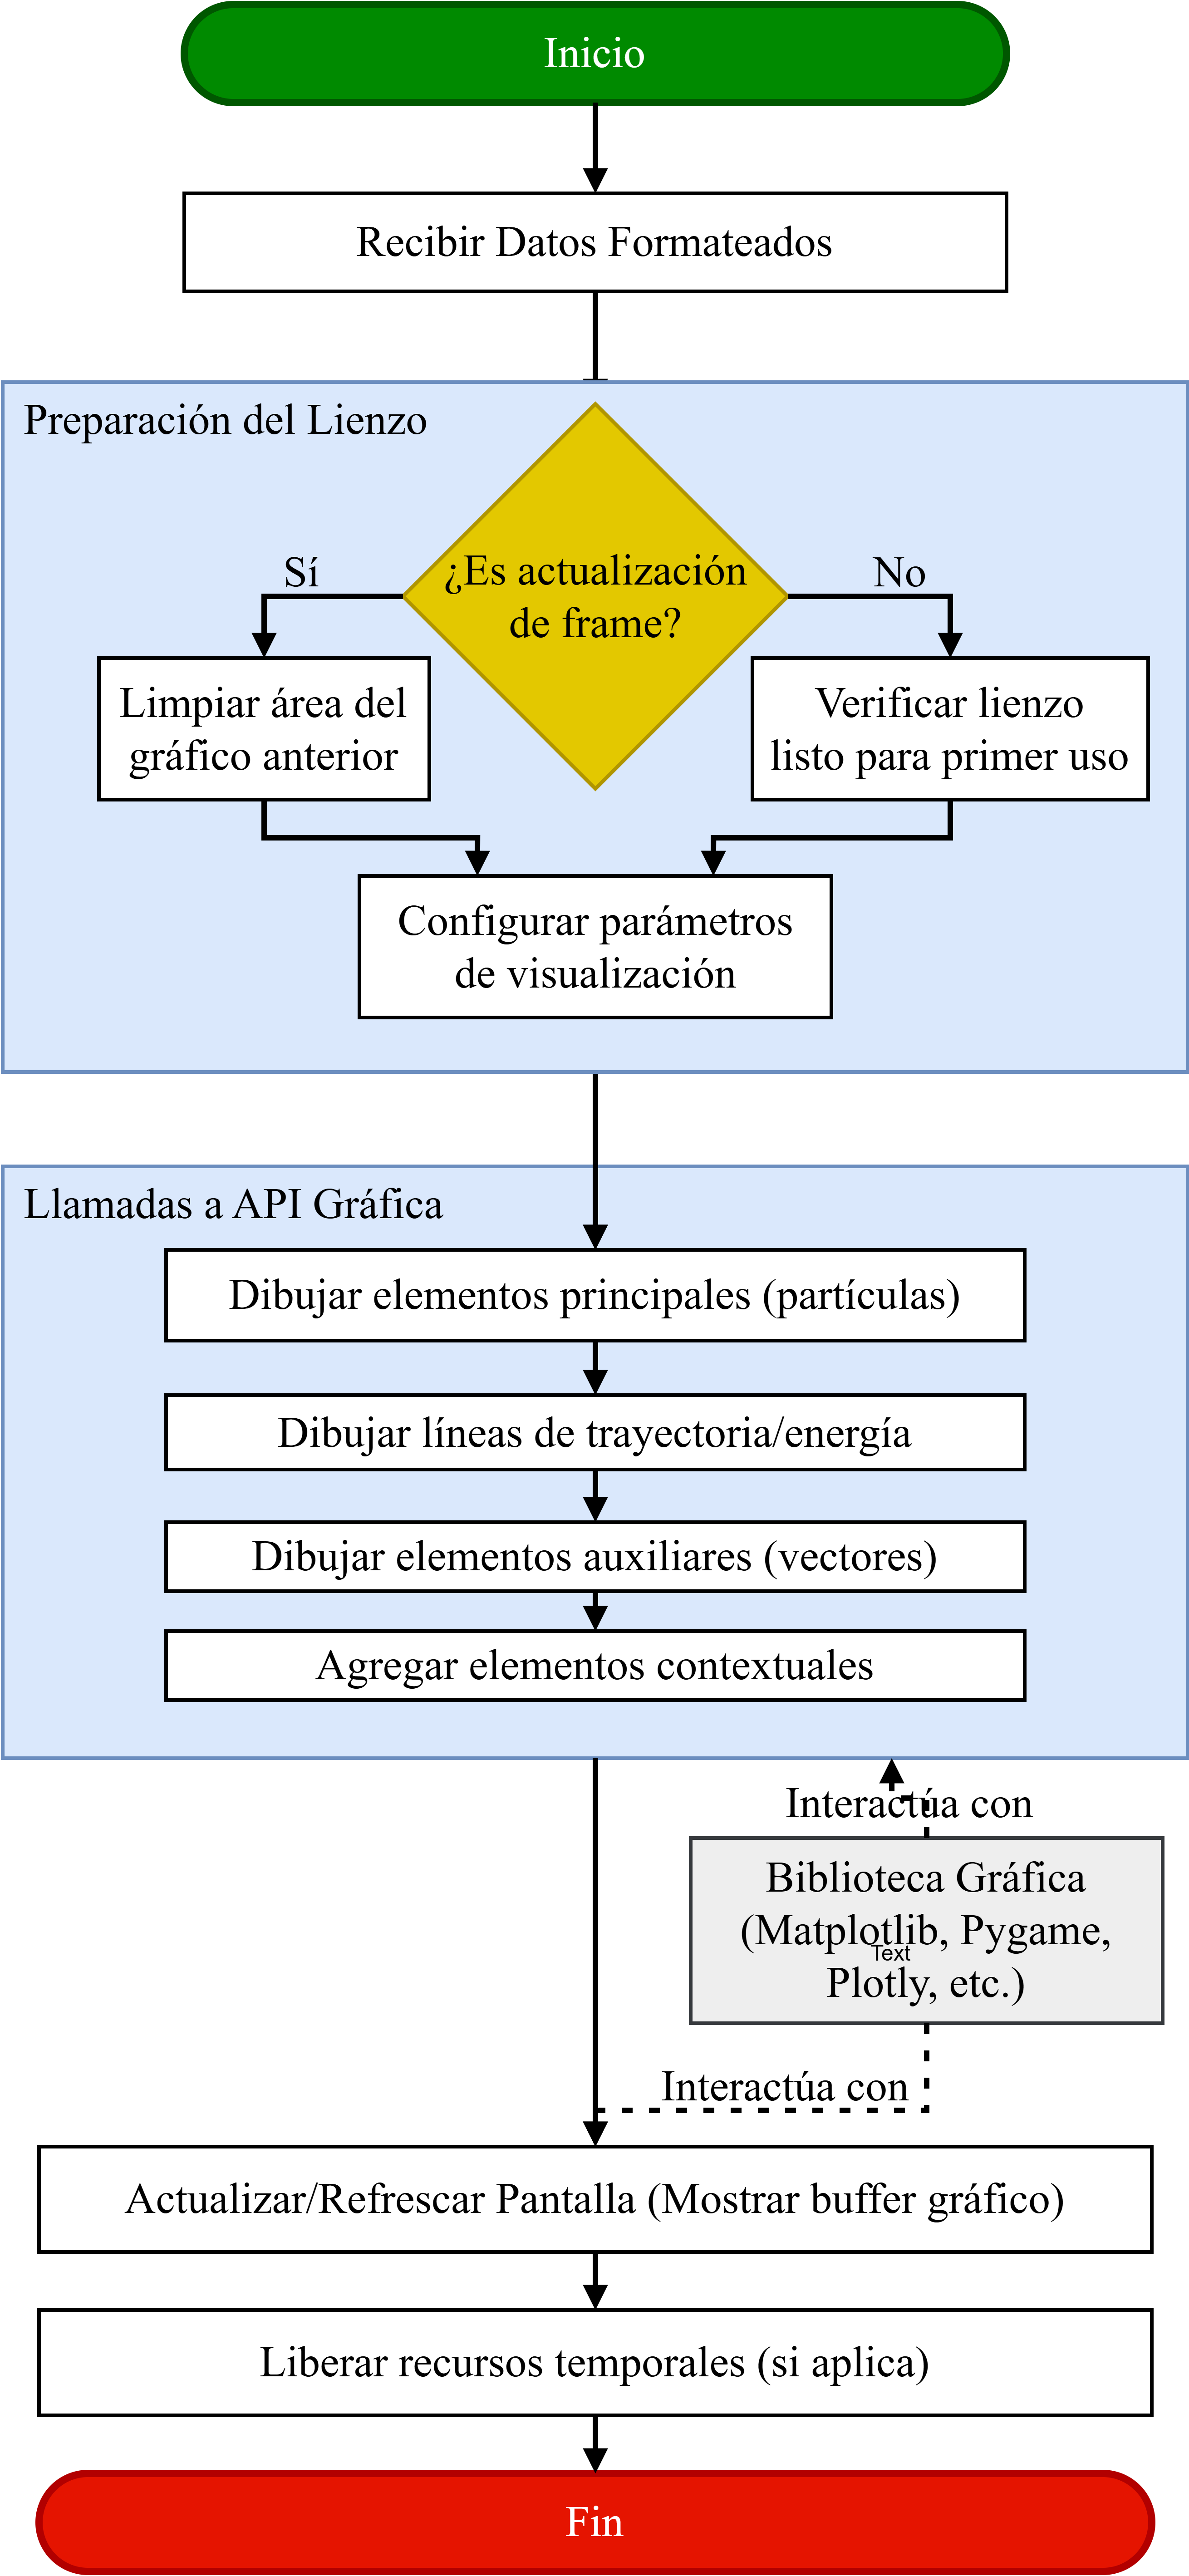
\includegraphics[width=\textwidth]{img/Analisis/DiagramaProcesos/DiagramaProceso12_GenerarGrafico.png}
    \caption{Diagrama de Proceso Interno 12: Generar Gráfico}%
    \label{fig:process_diagram12}
\end{figure}

\begin{figure}[H]
    \centering
    \includegraphics[width=\textwidth]{img/Analisis/DiagramaProcesos/DiagramaProceso13_CalcularFitness.png}
    \caption{Diagrama de Proceso Interno 13: Calcular Fitness}%
    \label{fig:process_diagram13}
\end{figure}

\begin{figure}[H]
    \centering
    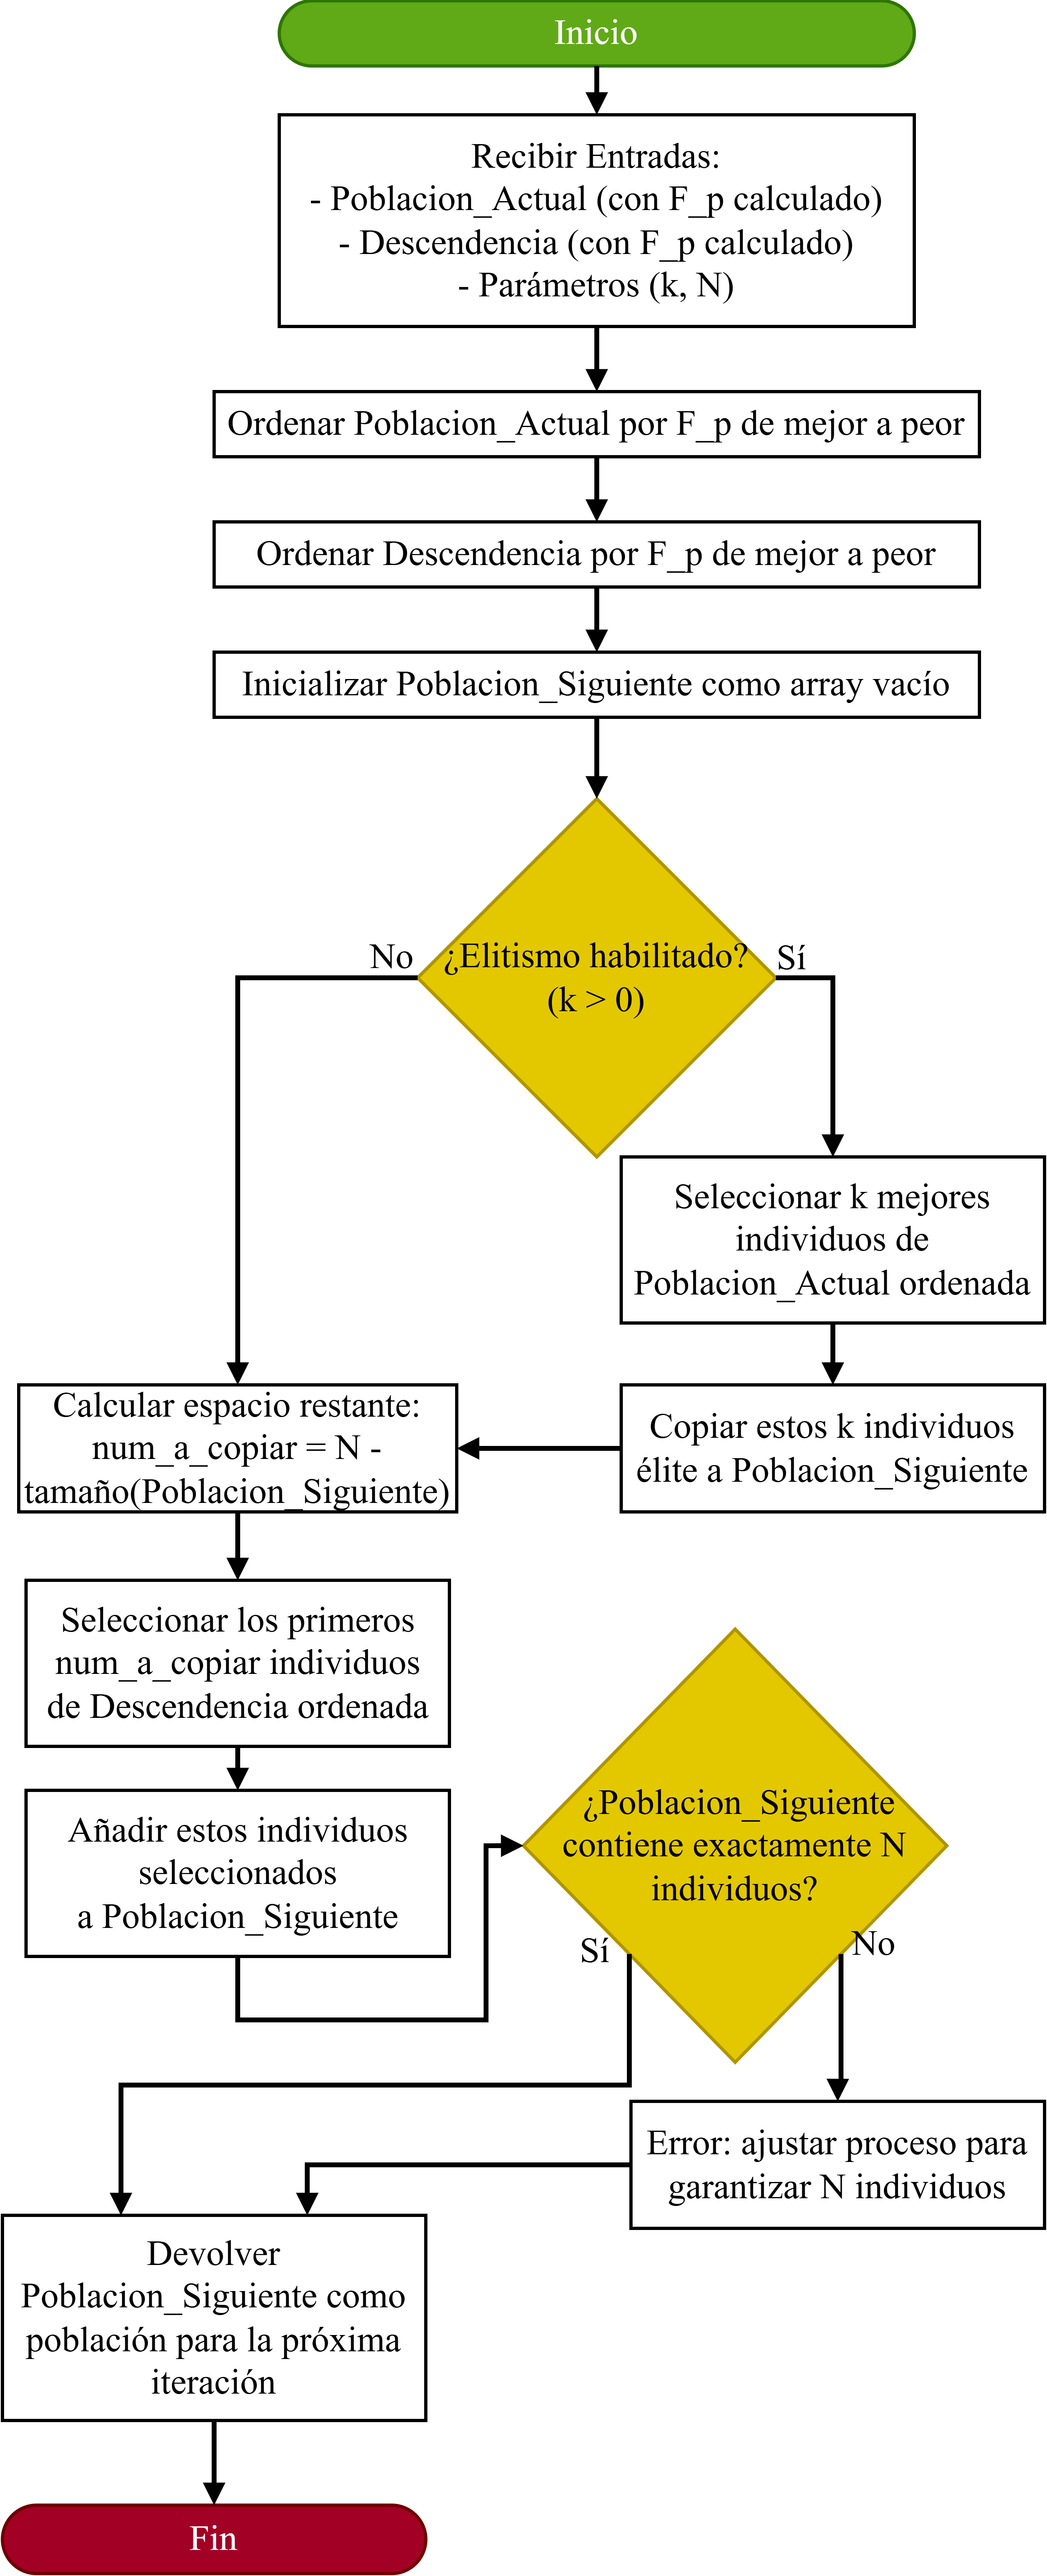
\includegraphics[width=\textwidth]{img/Analisis/DiagramaProcesos/DiagramaProceso14_SeleccionIndividuos.png}
    \caption{Diagrama de Proceso Interno 14: Selección de Individuos}%
    \label{fig:process_diagram14}
\end{figure}

\begin{figure}[H]
    \centering
    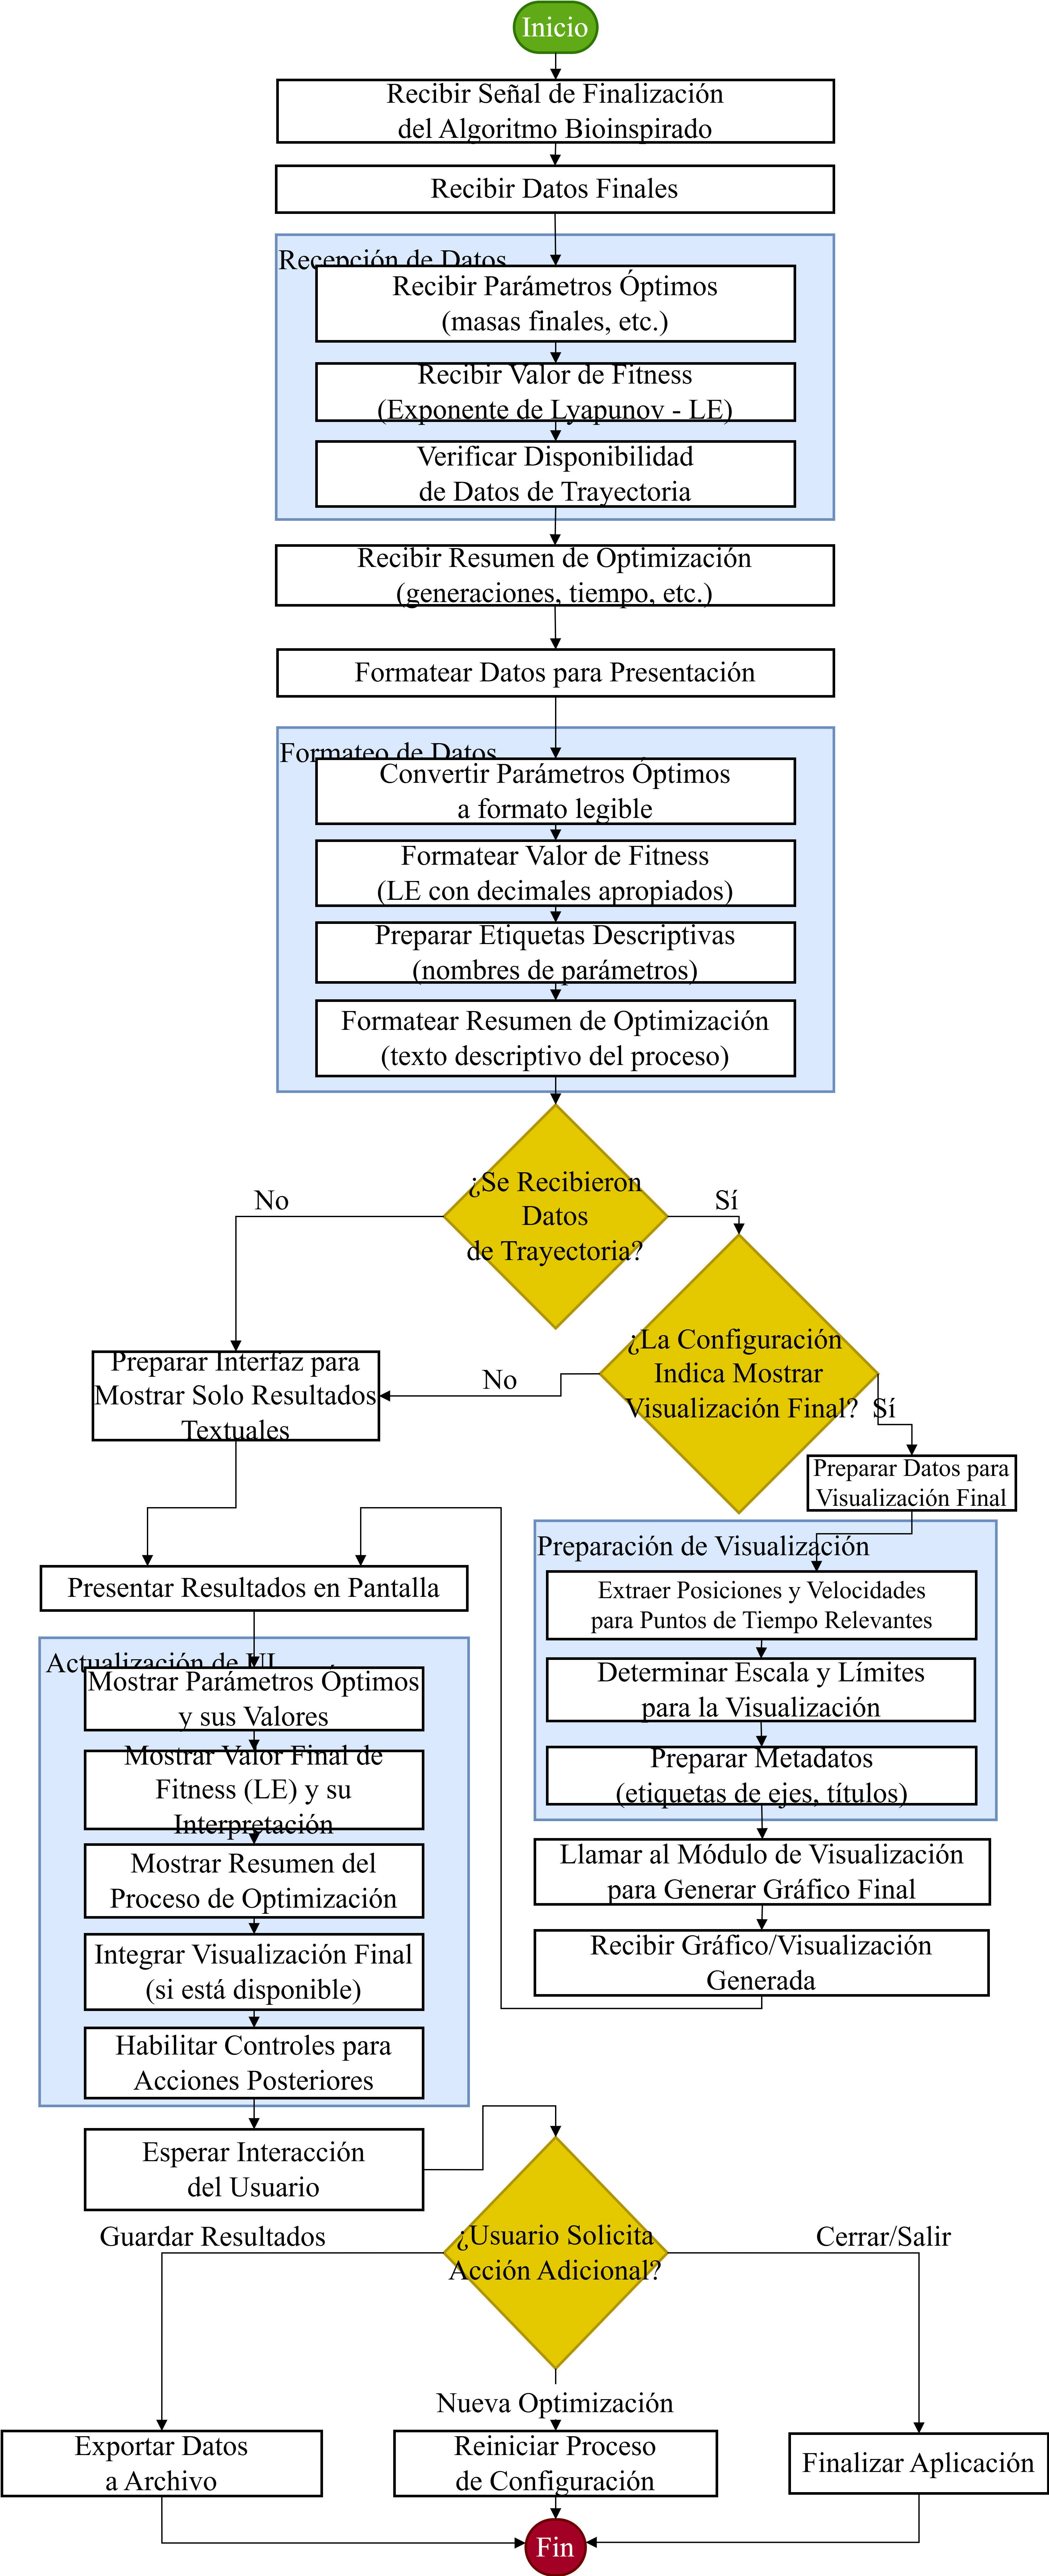
\includegraphics[width=\textwidth]{img/Analisis/DiagramaProcesos/DiagramaProceso15_Proceso Interno_Mostrar Resultados.png}
    \caption{Diagrama de Proceso Interno 15: Mostrar Resultados}%
    \label{fig:process_diagram15}
\end{figure}